\externaldocument{Evaluation.tex}
\chapter{Data processing for barcode detection}
\label{sec:Data processing for barcode detection}

\section{Overview}
\label{sec:Overview}
The system for detection of barcodes is basically divided in two parts. The data consist of a large amount of images which contain 1D- and 2D-codes. Figure \ref{barcodes} illustrates a typical data sample which contains different codes. Each image has a corresponding ground truth where the parts of the image containing codes have been labeled as "true" and the rest as "false".

\begin{figure}[H]
\centering
	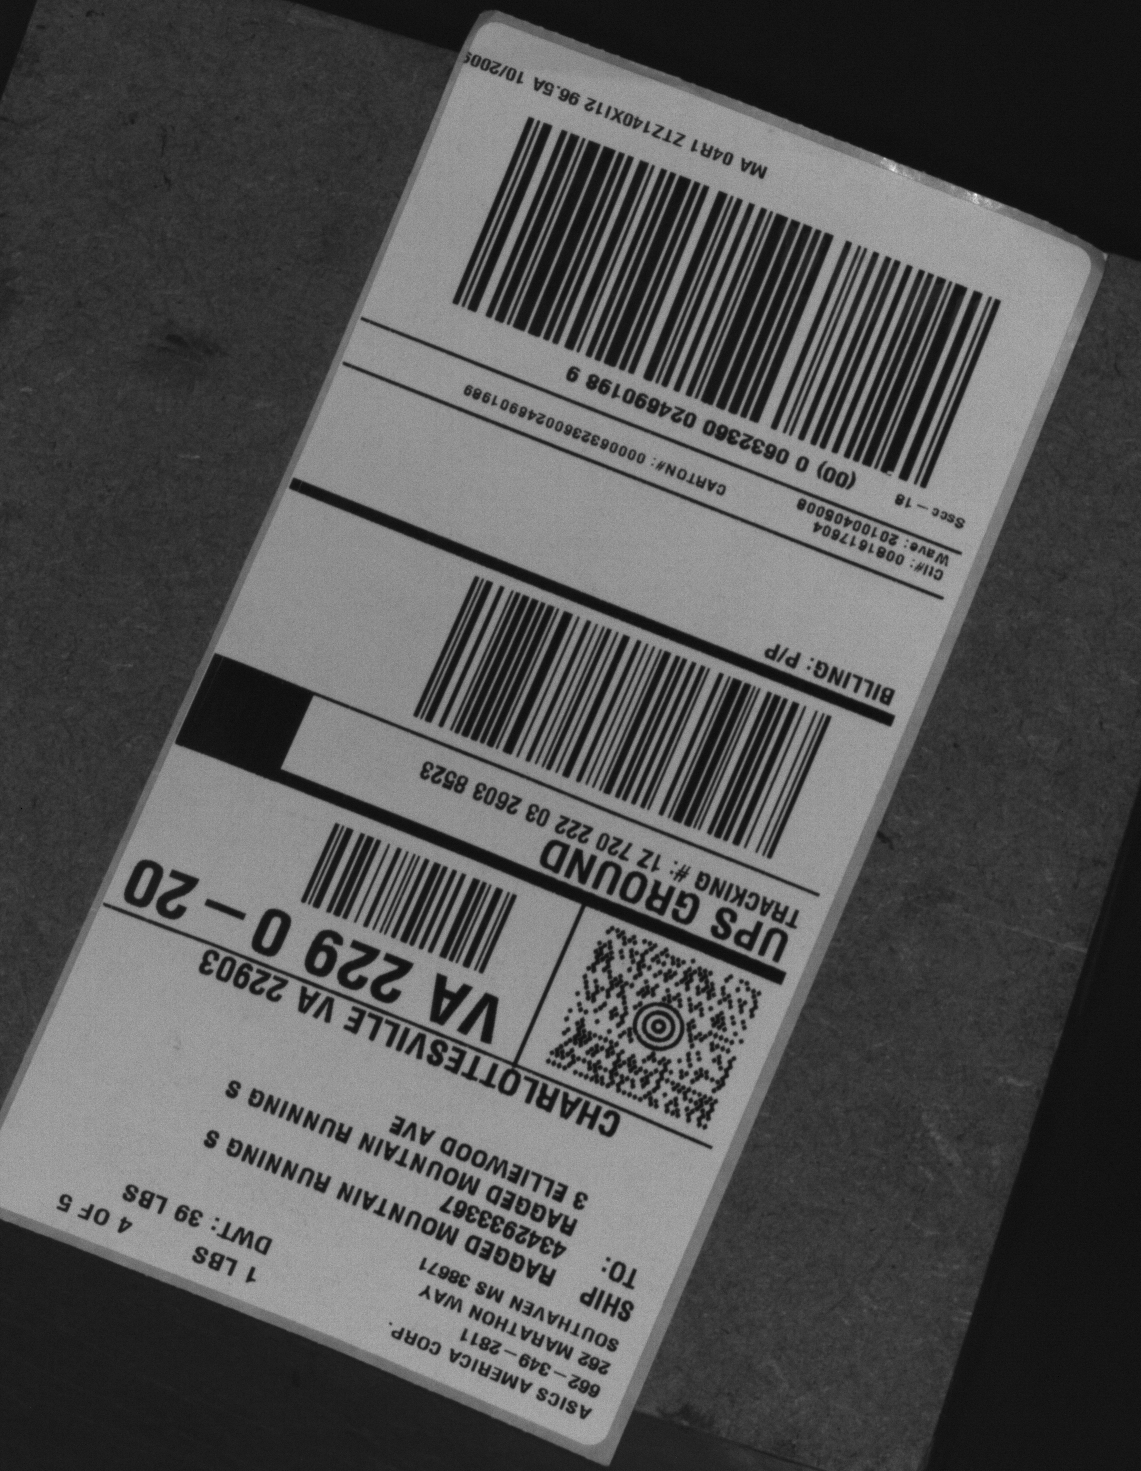
\includegraphics[scale=0.2] {barcodes}
	\caption{Image containing different types of codes}
	\label{barcodes}
\end{figure}

The first part of the system involves training using machine learning which produces a classifier. It consists of the following steps.
 
\begin{itemize}
	\item Preprocessing of images.
	\item Divide images and ground truth into tiles.
	\item Calculate features for each tile.
	\item Use machine learning to train the dataset.
\end{itemize}

The objective of the second part of the system is to predict unlabeled data as fast as possible. This is done with the trained classifiers and a cascade. It involves the following steps:

\begin{itemize}
	\item Preprocessing of image.
	\item In each step of the cascade calculate some specific features.
	\item Use the corresponding classifier for each feature to reduce the amount of data between each step in the cascade.
	\item Postprocessing of the output.
\end{itemize}
An overview of the system can be seen in \ref{system}.

%Flow chart
\begin{figure}[H]
\centering
\tikzstyle{largeblock} = [rectangle, draw, fill=blue!20, 
    text width=10em, text centered, rounded corners, minimum height=5em]
\tikzstyle{block} = [rectangle, draw, fill=blue!20, 
    text width=5em, text centered, rounded corners, minimum height=4em]
\tikzstyle{line} = [draw, -latex']
\tikzstyle{cloud} = [draw, ellipse,fill=red!20, node distance=3cm,
    minimum height=2em]
    
\begin{tikzpicture}[node distance = 2.5cm, auto]
    % Place nodes
    \node [cloud] (training) {labeled training data};
    \node [largeblock, below of=training] (machine) {training using machine learning};
    \node [block, below of=machine] (classifier) {classifier};
    \node [cloud, right of=training, node distance=4cm] (test) {test data};
    \node [block, below of=test, node distance=5cm] (cascade) {cascade};
    \node [block, below of=cascade] (prediction) {prediction};
    
    
    % Draw edges
    \path [line] (training) -- (machine);
    \path [line] (machine) -- (classifier);
    \path [line] (classifier) -- (cascade);
    \path [line] (test) -- (cascade);
    \path [line] (cascade) -- (prediction);

\end{tikzpicture}
\caption{Overview of the system}
\label{system}
\end{figure}

\section{Dataset}
\label{Dataset}
The dataset consists of a large amount of gray scale images containing 1D- and 2D-codes of different sizes and orientation. For each image the corresponding ground truth are also available. The images are first of all divided into one training dataset and one testing dataset. Each image is then divided into tiles of the same size: 
\begin{center}
\begin{equation}
	x = [x_1,...,x_N]
\end{equation}
\end{center}
With corresponding ground truth:
\begin{center}
\begin{equation}
	y = [y_1,...,y_N]
\end{equation}
\end{center}
The tiles can either overlap each other or just lay next to each other. For each tile a number of different features are calculated, i.e. each tile consists of a feature vector:
\begin{center}
\begin{equation}
	x_i =  
	\begin{pmatrix}
		 f_1 \\ \vdots \\ f_M
	\end{pmatrix}
\end{equation}
\end{center}  

\section{Preprocessing}
\label{Preprocessing}
Both during training and testing some preprocessing is applied to the images.

\subsection{Sharpening}
Some of the features used in the system gives better result with some sharpening. The reason for this is that the codes in some of the images have less contrast than others. Here a Laplace filter is applied to the images to make them a bit sharper. However some of the features gives better result without any preprocessing, therefore the filtered images are only used for calculation of some of the features.

\subsection{Down sampling}
All the feature used for code detection are more computational for larger tiles. Obviously a large amount of tiles also leads to more computations. For that reason a good idea can be to first down sample the image before dividing it into tiles. This will lead to less amount of tiles and less computations. However, down sampling the image could also lead to less accuracy. This has been evaluated in \ref{sec:Evaluation of barcode detection}.

\subsection{Overlapping tiles}
One alternative is to use overlapping tiles. This could lead to higher accuracy but the amount of tiles will increase which will lead to more computations. If the tile is too large it is necessary to use some overlap since some of the codes will not be detected otherwise. This if further explained and evaluated in section \ref{sec:Evaluation of barcode detection}.

\section{Postprocessing}
\label{Postprocessing}
At the end of the cascade when all the test data have been predicted there are some postprocessing before obtaining the final result. The reason for this is to remove some possible false classifications. The false classifications are often distinctive since the true positive classifications usually lay in clusters. Here a filter is applied which removes isolated true classifications. After that some morphological operations are done to fill some possible holes in the areas where the codes are.

\section{Code detection with AdaBoost}
\label{sec:Code detection with AdaBoost}
The system for code detection was first tried out with AdaBoost. If the system is going to be able to work in real time it has to be as fast as possible. One effective way to speed it up is to use a cascade when predicting the data. In the cascade one or several features are calculated at each step. In each step the corresponding classifier of the feature is used to classify the data. If the data is classified as true it will continue to the next step otherwise it will not be used any more. In the figure \ref{Cascade} the principle of the cascade is illustrated.

\begin{figure}[H]
\centering
\tikzstyle{block} = [rectangle, draw, fill=blue!20, 
    text width=5em, text centered, rounded corners, minimum height=4em]
\tikzstyle{datablock} = [rectangle, draw, fill=blue!20, 
    text width=5em, text centered, minimum height=8em]
\tikzstyle{line} = [draw, -latex']
\tikzstyle{predict} = [text centered]

\begin{tikzpicture}[node distance = 2.5cm, auto]
    % Place nodes
    \node [datablock] (test) {test data};
    \node [block, right of=test] (feature1) {feature 1};
    \node [block, right of=feature1] (feature2) {feature 2};
  	\node [block, right of=feature2] (feature3) {feature 3};
  	\node [predict, right of=feature3] (true) {true};
  	\node [predict, below of=feature1] (false1) {false};
  	\node [predict, below of=feature2] (false2) {false};
  	\node [predict, below of=feature3] (false3) {false};
       
    % Draw edges
    \path [line] (test) -- (feature1);
    \path [line] (feature1) -- (feature2);
    \path [line] (feature2) -- (feature3);
    \path [line] (feature3) -- (true);
    \path [line] (feature1) -- (false1);
    \path [line] (feature2) -- (false2);
    \path [line] (feature3) -- (false3);

\end{tikzpicture}
\caption{Cascade model}
\label{Cascade}
\end{figure}

An AdaBoost classifier is only able to handle two classes, true and false. Since the images contain both 1D- and 2D-codes it is necessary to separate them in some way. This is an other reason to use a cascade where one of the steps is to separate 1D- and 2D-codes. 

One good feature to use for this is the structure tensor. When only standard deviation and structure tensor is used to detect 1D-codes the following result is obtained. Figure \ref{codesepi1d1D} shows the amount of 1D-codes detected in each image and figure \ref{codesepi1d2D} shows the amount of 2D-codes detected. The result shows that structure tensor finds most of the 1D-codes and leaves out most of the 2D-codes.

\begin{figure}[H]
\centering
	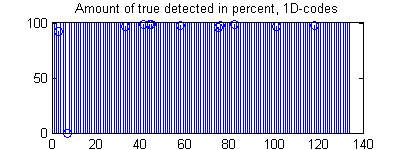
\includegraphics {codesepi1d1D}
	\caption{Amount of true detections for 1D-codes after using standard deviation and structure tensor classifiers}
	\label{codesepi1d1D}
\end{figure}

\begin{figure}[H]
\centering
	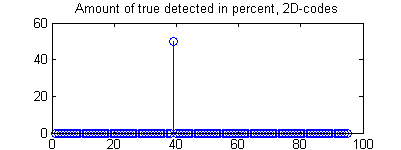
\includegraphics {codesepi1d2D}
	\caption{Amount of true detections for 2D-codes after using standard deviation and structure tensor classifiers}
	\label{codesepi1d2D}
\end{figure}

An other good feature to separate 1D- and 2D-codes is the FAST corner detection. Here only standard deviation and FAST corner detection have been used to detect 2D-codes. The amount of detections for 1D- and 2D-codes are shown in figure \ref{codesepFAST1D} and figure \ref{codesepFAST2D}.
\begin{figure}[H]
\centering
	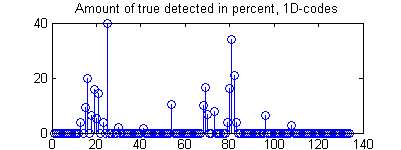
\includegraphics {codesepFAST1D}
	\caption{Amount of true detections for 1D-codes after using standard deviation and FAST classifiers}
	\label{codesepFAST1D}
\end{figure}

\begin{figure}[H]
\centering
	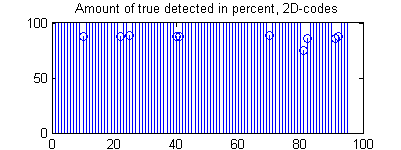
\includegraphics {codesepFAST2D}
	\caption{Amount of true detections for 2D-codes after using standard deviation and FAST classifiers}
	\label{codesepFAST2D}
\end{figure}

By testing different setups the cascade in \ref{Cascade1} has given good results. Here the standard deviation is calculated first. This feature is not very heavy computationally and it also reduces the amount of data quite a lot. In the second step the structure tensor has been used for separating 1D-codes from 2D-codes. In the last step the most computationally heavy methods are used.  

\begin{figure}[H]
\centering
\tikzstyle{block} = [rectangle, draw, fill=blue!20, 
    text width=5em, text centered, rounded corners, minimum height=4em]
\tikzstyle{datablock} = [rectangle, draw, fill=blue!20, 
    text width=5em, text centered, minimum height=8em]
\tikzstyle{line} = [draw, -latex']
\tikzstyle{predict} = [text centered]

\begin{tikzpicture}[node distance = 2.5cm, auto]
    % Place nodes
    \node [datablock] (test) {test data};
    \node [block, right of=test] (std) {Standard deviation};
    \node [block, right of=std] (tensor) {Structure tensor};
  	\node [block, right of=tensor] (dist) {Distance map};
  	\node [block, below of=tensor] (fast) {FAST};
  	\node [block, right of=fast] (LBP) {LBP};
  	\node [predict, right of=dist] (1d) {1D-code};
  	\node [predict, right of=LBP] (2d) {2D-code};
  	\node [predict, below of=std] (false1) {false};
  	\node [predict, above of=dist] (false2) {false};
  	\node [predict, below of=fast] (false3) {false};
  	\node [predict, below of=LBP] (false4) {false};
       
    % Draw edges
    \path [line] (test) -- (std);
    \path [line] (std) -- (tensor);
    \path [line] (tensor) -- (dist);
    \path [line] (tensor) -- (fast);
    \path [line] (fast) -- (LBP);
    \path [line] (std) -- (false1);
    \path [line] (dist) -- (false2);
    \path [line] (fast) -- (false3);
    \path [line] (LBP) -- (false4);
    \path [line] (LBP) -- (2d);
    \path [line] (dist) -- (1d);

\end{tikzpicture}
\caption{Cascade model 1 for code detection with AdaBoost}
\label{Cascade1}
\end{figure}

An other alternative is to use the FAST corner detection in the second step instead of the structure tensor. This cascade model is illustrated in \ref{Cascade2}

\begin{figure}[H]
\centering
\tikzstyle{block} = [rectangle, draw, fill=blue!20, 
    text width=5em, text centered, rounded corners, minimum height=4em]
\tikzstyle{datablock} = [rectangle, draw, fill=blue!20, 
    text width=5em, text centered, minimum height=8em]
\tikzstyle{line} = [draw, -latex']
\tikzstyle{predict} = [text centered]

\begin{tikzpicture}[node distance = 2.5cm, auto]
    % Place nodes
    \node [datablock] (test) {test data};
    \node [block, right of=test] (std) {Standard deviation};
    \node [block, right of=std] (fast) {FAST};
  	\node [block, right of=fast] (LBP) {LBP};
  	\node [block, below of=fast] (tensor) {Structure tensor};
  	\node [block, right of=tensor] (dist) {Distance map};
  	\node [predict, right of=dist] (1d) {1D-code};
  	\node [predict, right of=LBP] (2d) {2D-code};
  	\node [predict, below of=std] (false1) {false};
  	\node [predict, above of=LBP] (false2) {false};
  	\node [predict, below of=tensor] (false3) {false};
  	\node [predict, below of=dist] (false4) {false};
       
    % Draw edges
    \path [line] (test) -- (std);
    \path [line] (std) -- (fast);
    \path [line] (fast) -- (LBP);
    \path [line] (fast) -- (tensor);
    \path [line] (tensor) -- (dist);
    \path [line] (std) -- (false1);
    \path [line] (LBP) -- (false2);
    \path [line] (tensor) -- (false3);
    \path [line] (dist) -- (false4);
    \path [line] (LBP) -- (2d);
    \path [line] (dist) -- (1d);

\end{tikzpicture}
\caption{Cascade model 2 for code detection with AdaBoost}
\label{Cascade2}
\end{figure}


\section{Code detection with Random forest}
\label{sec:Code detection with Random forest}
Random forest and AdaBoost works in completely different ways when it comes to how the samples and the features are used. When using Random forest the cascade models in section \ref{sec:Code detection with AdaBoost} would not be a good choice. All the classifiers in the models except Local binary pattern only uses a few features. This would not be optimal when training a Random forest classifier. One characteristic thing with the Random forest algorithm is that it only uses a small part of all features in every split, this makes the trees in the forest more uncorrelated to each other.

One advantage with Random forest is that it is able to handle more than two classes. This can be utilized when using it for code detection since the images contain both 1D- and 2D-codes. One possible way would be to simply train one classifier with all features. However this would not be very effective since it is already known that some features are more computational than others. It is also known that standard deviation is an effective way to remove false tiles. For that reason Standard deviation has been used separately in the same way as in section \ref{sec:Code detection with AdaBoost} and the rest of the features are used in one classifier.

\begin{figure}[H]
\centering
\tikzstyle{block} = [rectangle, draw, fill=blue!20, 
    text width=5em, text centered, rounded corners, minimum height=4em]
\tikzstyle{datablock} = [rectangle, draw, fill=blue!20, 
    text width=5em, text centered, minimum height=8em]
\tikzstyle{largeblock} = [rectangle, draw, fill=blue!20, 
    text width=5em, text centered, rounded corners, minimum height=8em]
\tikzstyle{line} = [draw, -latex']
\tikzstyle{predict} = [text centered]

\begin{tikzpicture}[node distance = 2.5cm, auto]
    % Place nodes
    \node [datablock] (test) {test data};
    \node [block, right of=test] (std) {Standard deviation};
    \node [largeblock, right of=std] (LBP) {Strucure tensor, FAST, 		LBP, Distance map};
 	\node [predict, above of=LBP] (1d) {1D-code};
  	\node [predict, right of=LBP] (2d) {2D-code};
  	\node [predict, below of=std] (false1) {false};
  	\node [predict, below of=LBP] (false2) {false};

       
    % Draw edges
    \path [line] (test) -- (std);
    \path [line] (std) -- (LBP);
    \path [line] (std) -- (false1);
    \path [line] (LBP) -- (false2);
    \path [line] (LBP) -- (2d);
    \path [line] (LBP) -- (1d);

\end{tikzpicture}
\caption{Cascade model for code detection with Random forest}
\label{Cascade3}
\end{figure}

% Local Variables:
% TeX-master: "main.tex"
% End:
